\documentclass[12pt]{article}
\usepackage[utf8]{inputenc}
\usepackage{indentfirst}
\usepackage{graphicx}
\usepackage{hyperref}
\hypersetup{
    colorlinks,
    citecolor=black,
    filecolor=black,
    linkcolor=red,
    urlcolor=blue,
}
\usepackage{subcaption}

\title{\textbf{Internship Report} \\ AC6}
\author{Cinquanta Octave \\ CY Tech Student}
\date{August 2021}

\begin{document}

\begin{figure}
    \captionsetup[subfigure]{labelformat=empty}
    \centering
    \subcaptionbox{}{%
        
\includegraphics[width=0.30\textwidth]{AC6.png}}\hfill
    \subcaptionbox{}{%
        
\includegraphics[width=0.30\textwidth]{CY_Tech.svg.png}}
\end{figure}

\maketitle

\section{Acknowledgements}

I wish to dedicate my work to my internship supervisor, Bernard Dautrevaux, for being an excellent supervisor during my time at AC6. I would also like to thank my colleagues, Kevin Tang, Tarek Lakbiri, Samuel Da Costa Ribeiro, Khalid Khatouri, Hakim Benhabiba, Ayoub Bourjilat and Roy Jamil, for their help and support during this internship, as well as Valerie Bagnaschino and Jean-Michel Grasser for kindly welcoming me amongst them for a while. I also wish to acknowledge my friends and family for their overall support.

\newpage
\section{Introduction}

For this last year of the Bachelor in Data Science, I obtained an internship at AC6, a company specializing in Embedded Systems. It took place in AC6's main offices located in Courbevoie. The internship started on the 1st of April and ended on the 31st of August, for an effective duration of 5 months. \\
The company's work did not align with my studies, but thankfully my supervisor managed to find work suitable for me at AC6.

\section{Summary}

Through this internship report, I will firstly provide details on how I found this particular internship. I will then proceed with an objective description of the company, first in general and within its sector of activity, then the various tools it utilizes, followed by a more subjective view of the company during my stay at AC6, an lastly how my incorporation within the company proceeded. The next section consists of a technical description of the various tasks I completed during my internship, followed by how those tasks were organized, how I managed to self-evaluate while working, and a discussion of the results of my work. Finally this report will conclude by looking at the impact of this internship on my studies, and vice-versa.

\newpage
\tableofcontents
\listoffigures

\section{Search for an Internship}

The search for an internship was a rather complex task this year. The difficulty of finding an internship mostly stemmed from the imposed limitations on the duration of said internship. The duration requested was of 4 to 5 months, meaning that the internship had to be a paid endeavour, as it was longer than the legal pay threshold of 2 months and a day, yet it had to be shorter than the most desired and practical internship length, 6 months. Another obstacle was that this internship was not at the very end of my studies, as another year of studying awaited me afterwards. This made obtaining an internship with the promise of either free labor or continuous labor with possibility of employment afterwards impossible. As such many companies I had applied for an internship at ended up either declining or not following through, and their choice was usually made with haste. I also tried to use my personal network to potentially obtain an internship despite not fitting into a company's desired intern profile, and as it did for my first two internships, it worked this time too. A relative introduced me to the director of a company working in embedded Linux. At first, he tried helping me find an internship within a company his had ties with, alas my specialization as a Data Scientist was too different from what those companies were seeking. In the end, he decided to give me an internship within his own company, where he would find appropriate tasks for me to perform, and provide me enough time to learn the ropes as well.

\newpage
\section{Internship Environment}

\subsection{Objective View of the Company}

\subsubsection{The Company}

AC6 was founded in 2003 by Bernard Dautrevaux and William Kazuro, and was originally named Acsys, which stands for Assistance Conseil Système. This name perfectly describes one of the three main sectors of services AC6 offers, which are : training courses, consulting and creation of integrated development environments (IDEs). AC6's main commercial activities all gravitate around Embedded Systems and their applications. Let us now have a detailed look at what those services are and how they operate. \\
The training courses are offered to other companies on a variety of subjects concerning embedded systems. Those courses usually last between 3 and 5 working days, and they can be taken wherever the client feels most comfortable taking the course, as such it can be done fully in the offices of AC6, completely online or even in the client's own offices. The courses can be taken by multiple employees of the same company at once, or even by employees from several different companies depending on the nature of the subject. The courses are also taught in English, and thus international companies can effortlessly follow, without the need to learn French. It is the job of the instructors to write, prepare and teach those courses. As it is a time consuming task but also the main source of income for the company, it is the priority of several employees to actively seek out contracts with different companies and then prepare the corresponding course if a contract is signed. \\
The consulting aspect of the company's services consists in accomplishing tasks and providing software at the request of another company. As such, this task also transcribes into various contracts happening on a non periodic basis. This service is usually provided by the engineers as well as the apprentices and interns present. A concrete example of what those services could be is for instance a company contracting AC6 to update their WiFi drivers for one of their new micro-controllers as to add compatibility with a particular version of Linux. These contracts therefore require various levels of skills and thus usually the cooperation of multiple employees to efficiently complete them. \\
The third and final sector of AC6's services is the development of IDEs, or more specifically the creation and maintenance of plugins that can be incorporated into an IDE. Such a plugin is System Workbench for STM32, an Eclipse plugin developed in cooperation with the research team of STMicroelectronics and maintained by AC6's developers. This plugin is used for the programming of STM class micro-controllers designed by STMicroelectronics, and as such they put together a partnership with AC6 for the plugin's development. The development team is currently working on another plugin for Eclipse called System Workbench for Linux, which should drastically simplify the creation of specific Linux builds for embedded systems. \\
AC6 currently has half a dozen permanent employees as well as several apprentices working under said employees. It is as such considered a very small company. The employees currently count a CEO, a secretary, an accountant, 3 engineers, of which a developer and 2 instructors, 3 apprentices and 2 interns. Its organization can also be represented as follows :

\begin{figure}[h]
    \centering
    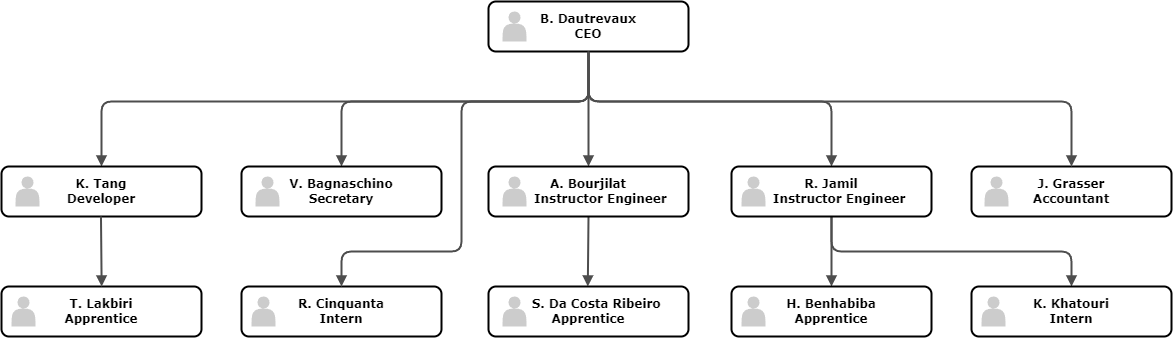
\includegraphics[width=\textwidth]{orga.png}
    \caption{Organizational Chart of AC6}
    \label{org}
\end{figure}

As previously stated, AC6 is partnered with STMicroelectronics to work on their microcontroller series STM32. It is also partnered as a consultant with NXP. AC6 employs the Tracealyzer tool made by Percepio to detect issues under certain embedded OSs. AC6 is a member of the ARM Connected Community and provides training for engineers on systems based on ARM technology. AC6 also supports various security tools such as wolfSSL, and Open Source development platforms such as the Yocto project and freeRTOS.

\newpage
\subsubsection{The Company's Tools}

AC6 employees mostly work under Linux systems, as they require this OS to be able to test and build the various libraries and distributions they work with. The apprentice in charge of designing the company's advertising assets and creating the promotional videos works with a high-end Mac Studio for its processing power. The main Integrated Development Environment they use to develop is based on Eclipse, for it is practical for project management and they are quite familiar with it, having developed their plugin for this IDE. To organize and allocate work between employees, they use a platform called Redmine, a project management website. This website allows them to create sub-projects, issue and tasks that can be documented and timestamped. This effectively allows for the company to keep track of who does what and when, along with how much time is spent on a particular issue. The various issues can be reviewed as a Gantt type chart for a clearer understanding of the work flow. The company also possesses its own local servers that the employees can use to store and share their work. The employees communicate using Skype for messages, as well as Microsoft Teams for online meetings.

\subsection{Personal View of the Company}

Due to the rather small size of the company, the relationships between the employees, no matter their title, aren't distant or non-existent as they would in a bigger company. Even an intern working under one of the employees knows and communicates with the CEO on regular occasions. The employees are divided into 2 rooms in which they work, one of them housing the CEO, the secretary and the accountant, and the other housing the engineers, the apprentices and the interns. Both rooms transpire their own professional yet comfortable mood, as banter between employees and discussions around lunch can be often heard. Sometimes the CEO might invite everyone to lunch, and use this opportunity to bring his employees up to speed concerning work or simply to help integrate newly arrived interns.

\subsection{Incorporation of the Student within the Company}

As the previous paragraph might imply, I was well integrated within the company, as everyone there welcomed me in a friendly manner. This incorporation happened at a rather good pace, each lunch spent discussing with my colleagues speeding up the process. At the end of the day, I ended up on good terms with every member of AC6, no matter whether they were someone I would work with or simply greet everyday. It mainly manifested as occasional banter with my colleagues, especially with the other intern and the apprentices, as our small age gaps made it easier to communicate. However, even though the 3 engineers were about 10 years older than I was, our common interests for Computer Science and other hobbies made breaking the ice easier. 

\section{Technical Intakes}

\subsection{Technical Description}

The environment I ended up working on was a Windows 10 distribution on a Lenovo computer. I was given the freedom to use whichever tools I preferred to develop with, and as such I chose to use Visual Code Studio as my IDE. I also used Github to host and preserve my work, and TeamViewer to remotely connect to my computer in case I could not go to the office. \\
Given the impromptu nature of my internship, my supervisor ended up deciding on the go what tasks he would assign me depending on his current needs. As such, I was assigned 3 different tasks during my time at AC6, and I shall now detail them in the following paragraphs. Each one of these tasks took roughly 6 weeks each, with an occasional overlaying of tasks and redirection of priorities. The tasks will also be followed by a diagram designed to facilitate the understanding of the structure of each one. \\
The first task I was given was the management of the company's DMARC reports. In order to fully understand this task, one first needs to know what a DMARC report is. When an email is sent, the email's data, as in recipient, sender, status, etc., is collected by specific email addresses linked to a domain. Those addresses' job is to compile the emails' data into DMARC reports and send these back to the domain owner, here AC6. The reports allow a domain owner to check whether their emails are getting through security checks, and if they aren't, which ones they failed. This allows for a better understanding of one's traffic, and thus provides a decent diagnostic tool for potential issues. However, for almost every mail or small group of mail is a report created, and the traffic of AC6 consists in more than 100,000 emails in a month, therefore it is impossible to make sense of such large data without proper filtering and analysis. This is where the task I was given comes in. The DMARC reports already had their own email address that would save the reports in a specific folder of an AC6 server. My task was to parse these reports using an algorithm, and using the obtained data, set up a dashboard of graphs that well summarized the state of the emails, such as how many passed and failed each tests, which country and domain they come from, their IP address, etc., all in an easy to read and interpret manner so that only a quick occasional check of the dashboard is necessary. The main algorithm was written in Python, and the data it parsed was sent to a MySQL database, who communicated with a dashboard set up using Grafana, an open source dashboard library, hosted locally. The presence of the SQL database allowed for easy data parsing and filtering, and a manual access to the data should the need arise. I had chosen to write the algorithm in Python as it is the language I felt most comfortable with, and it was well suited for the job. Most of the testing for this task was done on a laptop specialized for Linux builds, as it was more consistent than Windows. \\

\begin{figure}[h]
    \centering
    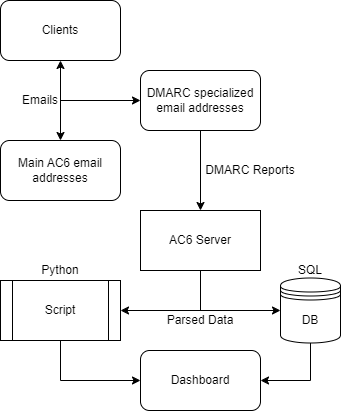
\includegraphics[width=0.55\textwidth]{dmarc.png}
    \caption{Diagram of the DMARC Report Analyzer}
    \label{dmarc}
\end{figure}

The second task I was given was helping with the management of the System Workbench for Linux licenses. The Eclipse plugin AC6 is currently working on, System Workbench for Linux, is sold as a license that activates the software and lets the consumer use it. The license however is not indefinite, and is usually sold as a period of one month or one year, and thus the software needs to be aware of when the license is expired and when to remind the user to extend their purchase. As such, there needs to exist a database of licenses that can communicate with the software in order to maintain up to date information on the client's side of things. Thus my second task was to create such a database and the means to communicate with the software. As such I built a database that would be linked with an API hosted by AC6, that the software would make HTTP requests to in order to obtain the information it needed. The software would use the client's MAC address and the license type to obtain the expiration date as well as the status of the license. The software would then act accordingly in managing the user's permissions. As the software was written in Java, I also wrote my algorithm in Java so it would be easy to incorporate within the software's code for its developer. The database was also a MySQL database, since the company is used to hosting such databases. The API was written in PHP, the language best suited for handling incoming HTTP requests, and the easiest with which an API can be set up. \\

\begin{figure}[h]
    \centering
    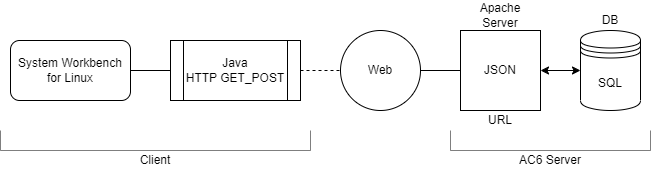
\includegraphics[width=\textwidth]{license.png}
    \caption{Diagram of the System Workbench License Manager}
    \label{sw4l}
\end{figure}

The third task was to create a mock-up of a new version of the AC6 website. This website was setup a long time ago, and as such my supervisor wanted to change its appearance to a more modern looking site. As such the apprentice in charge of any designing work was tasked with visually creating the website using elements of the old one, and I was to work with him by programming the various images he would draw. However, we would usually be quite limited in terms of how much we could do, as AC6 did not want to spend too much resources crafting the website, and as the designer had never done any web development, he had no idea whether something fancy was easy to do or not worth the time, and as such I had to guide him, giving him as much feedback as I could along the way. The most complicated aspect of this task was trying to make a responsive website, aka a website that adapts to the format of the screen it is seen through, as such it should look as good on a computer as on a phone. This is generally a difficult task, and for someone like me with practically no web development skills, it is hardly feasible. The mock-up was written in HTML 5, with CSS for the appearance and Javascript for certain functionalities. Given the nature of the website as HTML blocks incorporated into a skeleton, a single page needed to be on a single file, without calling any external script or library.

\begin{figure}[h]
    \centering
    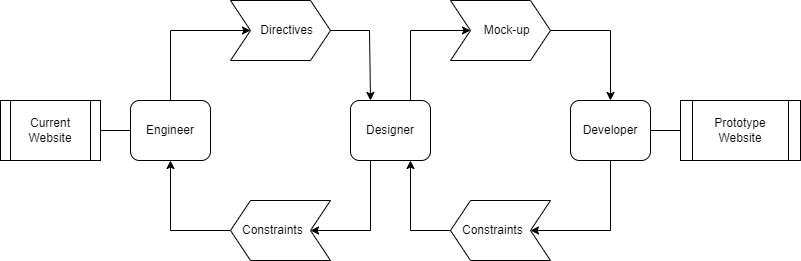
\includegraphics[width=\textwidth]{website.png}
    \caption{Diagram of the Website Creation Process}
    \label{web}
\end{figure}

\subsection{Organization}

During the internship, my desk was placed in the room that contained the engineers and apprentices, and as such they would be the ones I spent most of the time with. My supervisor was in another room, however I would still often consult him to make sure I was progressing in the right direction. The tasks I was assigned had me collaborate particularly with System Workbench for Linux's lead developer and the apprentice working as a designer. I was never set specific deadlines other than all my tasks needed to be accomplished before the end of my internship. The tasks I had were set up on Redmine along with deadlines, but these were simply to have an idea of approximately when any task would be done, these were not hard deadlines. 

\subsection{Self Assessment}

For any given task, I would usually first receive a global briefing of my supervisor's expectations and the various constraints I would face going forward. Then I would start working on the task, and regularly keep my supervisor up to date with how I was faring, so that he would be able to tell me whether I was doing things correctly or actually taking a wrong turn without realising it. Depending on the task, these update could go from being daily to weekly. When it comes to quality of work, I tried to write code as efficiently as possible, and minimize the overhead running the algorithms would generate. 

\subsection{Results and Potential Continuation}

The tasks I was given were accomplished, although the third one not to the extent I would have wished for it to be. The DMARC report analyzer should be available to be put to use directly from the server files where I deposited it, and thus can be run whenever my supervisor desires to check the dashboard. The System Workbench License Manager files were given to my colleagues, one of them managing to reproduce the hosting of the database and the other the integration of my function to the main software code, thus it has been incorporated into the company's work. The Website Mock-up was not as qualitative as it should have been, it is however still something that can be built on, and I would guess that my supervisor plans to work on that front himself, as he was the one to design the old website in the first place. I would like to check up on the members of AC6 in the future, however, when it comes to my next internship or apprenticeship, I wish for it to be in a company specifically looking for a data scientist.

\section{Internship within my Studies}

As this internship was set in a company dealing with embedded systems, a subject I have never been taught on, and the tasks I was given apart from the first were rather foreign to my studies, the lessons I had been taught by the school were not exactly of any help here. The data parsing of the first task was the exception to that statement. Apart from that, I had to rely on my general knowledge of programming and a good deal of improvising. The unfamiliarity of my tasks served however in teaching many things I would never even approach during my studies, such as API hosting and web development. As such this internship was an excellent opportunity for me to learn diverse knowledge, as well as the life of a small company.

\section{Conclusion}

In the end, this internship was a good experience. I managed to learn a great many things while still maintaining a decent productivity for the company. Despite the obvious mismatch between the company's main sector of activity and my studies, I was able to successfully complete this internship, mainly due to the warmhearted welcome I received.

\section{Bibliography}

\begin{itemize}
    \item Information provided by my internship supervisor and colleagues
    \item \url{https://www.ac6.fr/}
    \item \url{https://www.st.com/content/st_com/en/partner/partner-program/partnerpage/AC6.html}
    \item \url{https://www.nxp.com/webapp/connect/displayPartnerProfile.sp?partnerId=1-9HXC-1}
\end{itemize}

\section{Annexes}

The entire source code for my work during this internship is available at \url{https://github.com/PurpleShad0w/ac6}.

\begin{figure}[h]
    \centering
    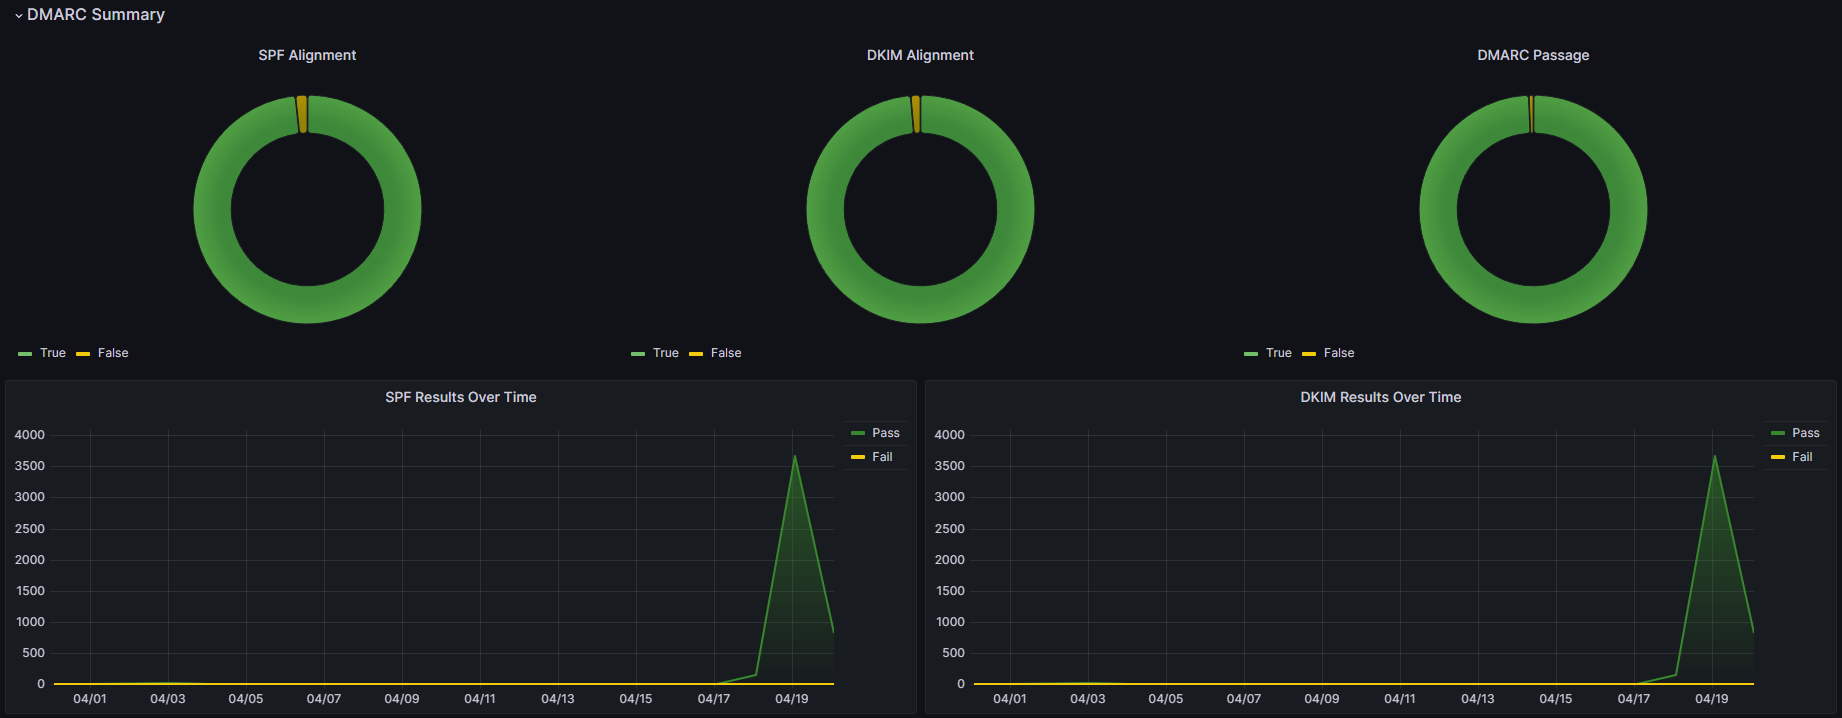
\includegraphics[width=\textwidth]{dashboard.png}
    \caption{DMARC Dashboard (1)}
    \label{dash}
\end{figure}

\begin{figure}[h]
    \centering
    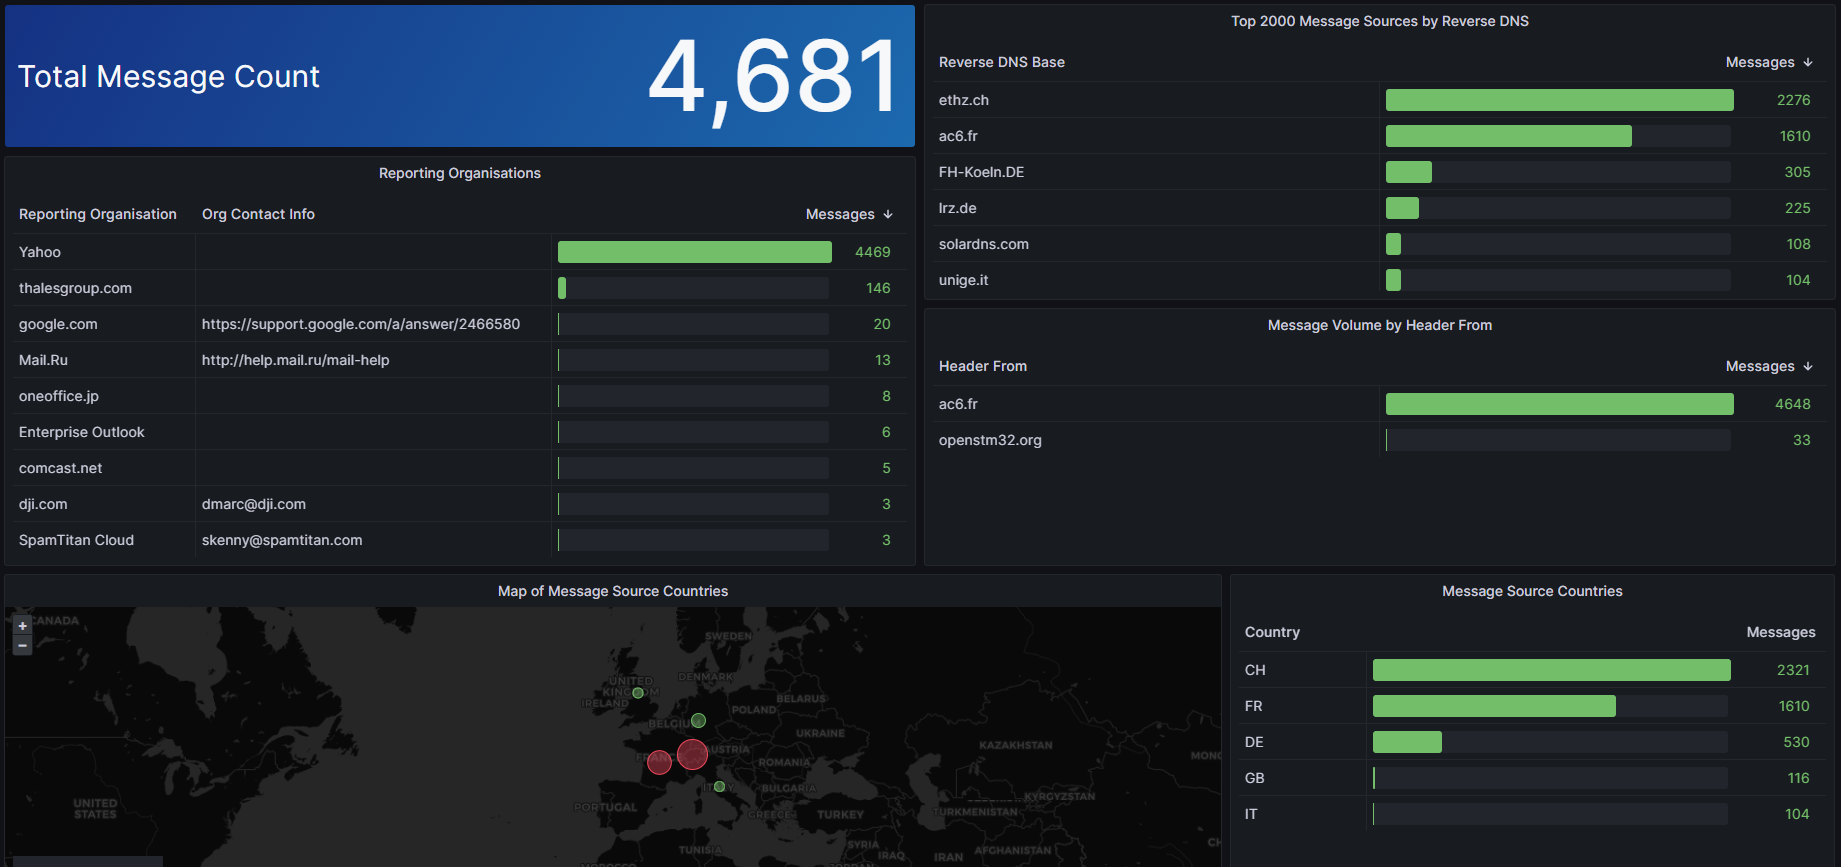
\includegraphics[width=\textwidth]{dashboard 2.png}
    \caption{DMARC Dashboard (2)}
    \label{dash2}
\end{figure}

\begin{figure}[h]
    \centering
    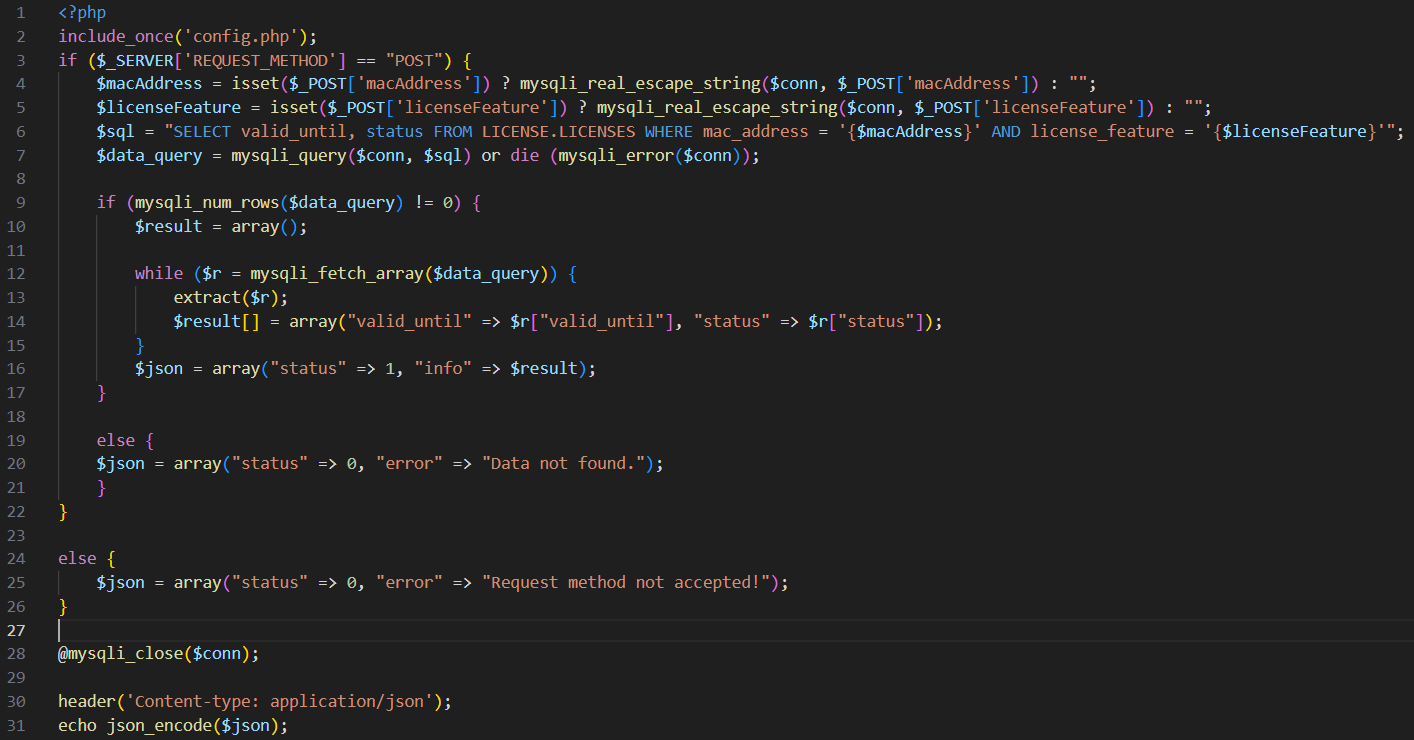
\includegraphics[width=\textwidth]{post.png}
    \caption{The PHP API source code}
    \label{post}
\end{figure}

\begin{figure}[h]
    \centering
    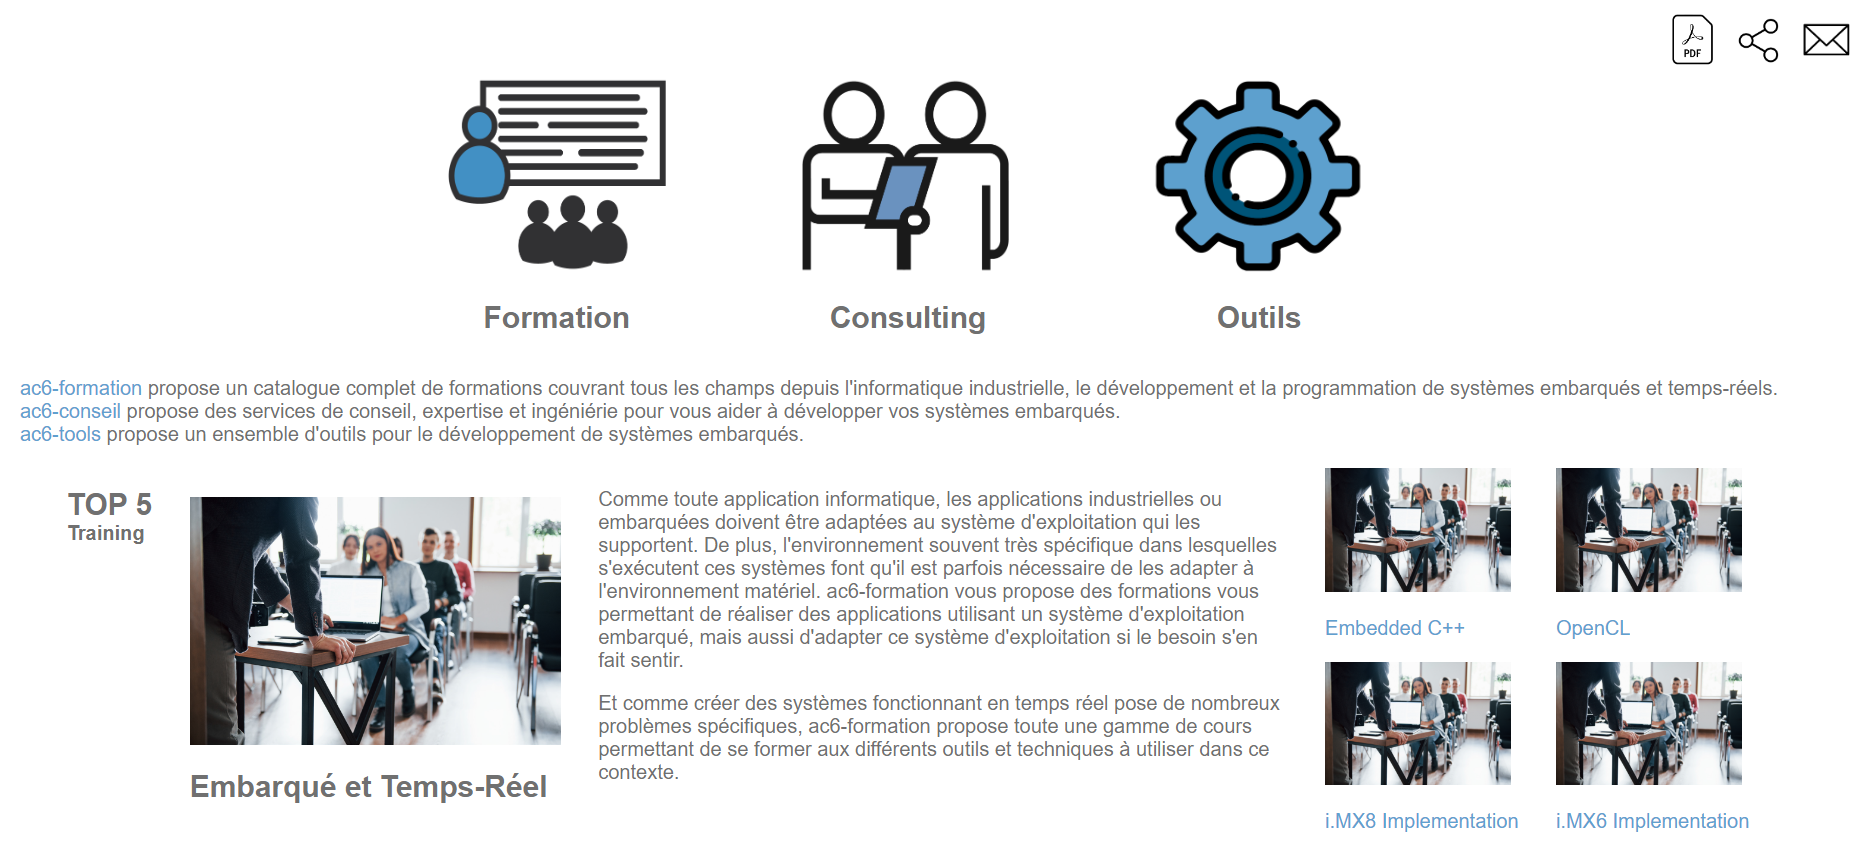
\includegraphics[width=\textwidth]{home.png}
    \caption{Website Mock-up - Homepage}
    \label{home}
\end{figure}

\begin{figure}[h]
    \centering
    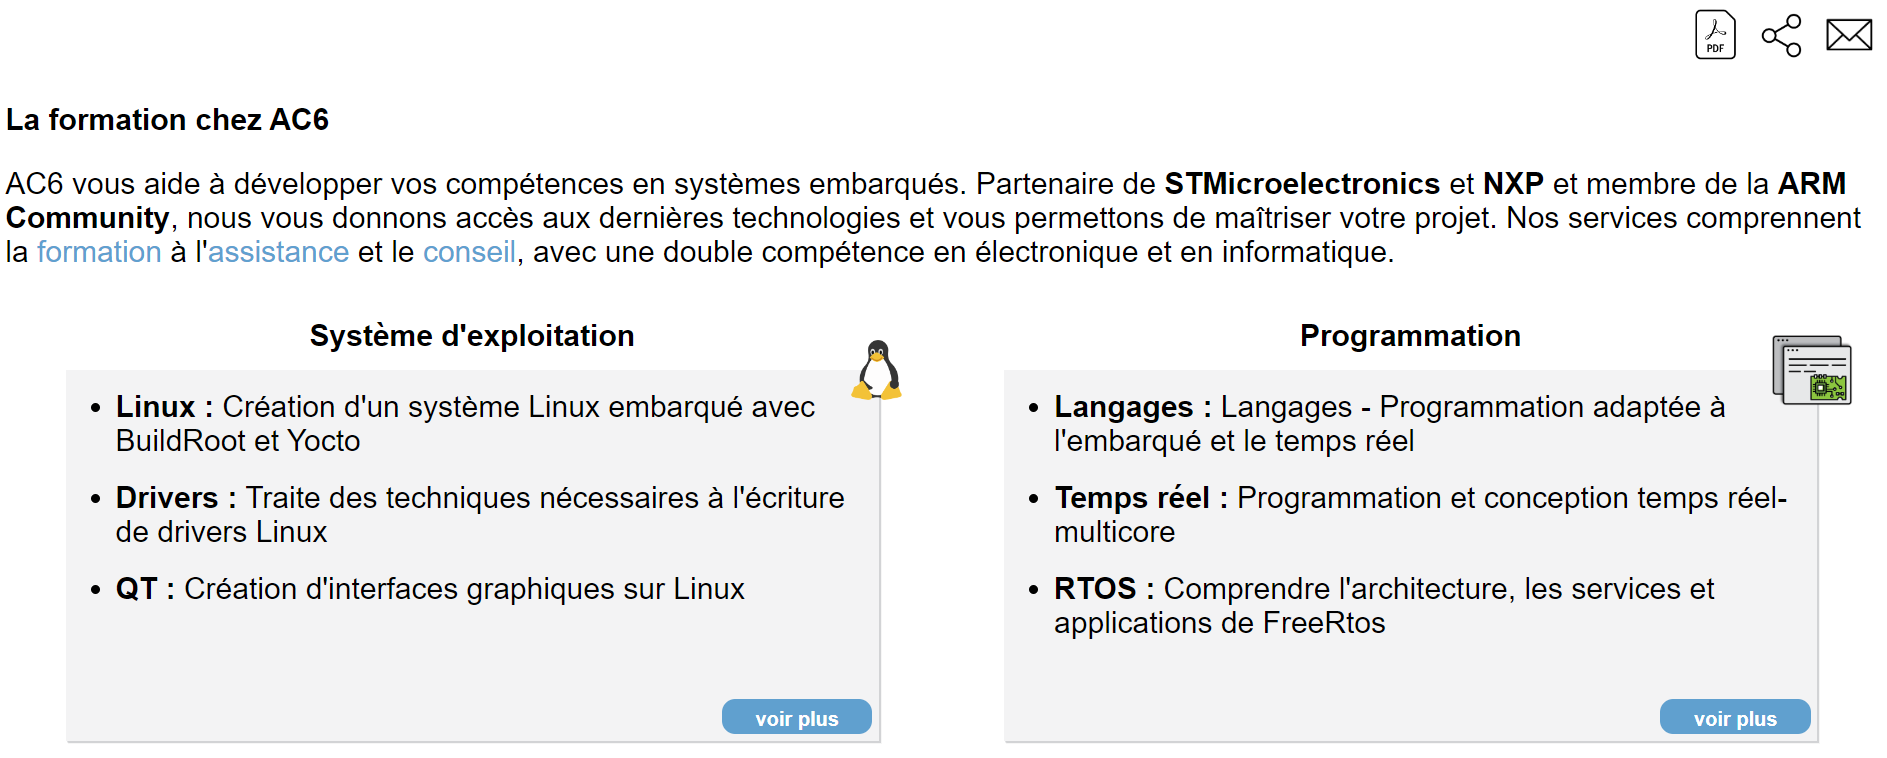
\includegraphics[width=\textwidth]{training.png}
    \caption{Website Mock-up - Training Page (1)}
    \label{training}
\end{figure}

\begin{figure}[h]
    \centering
    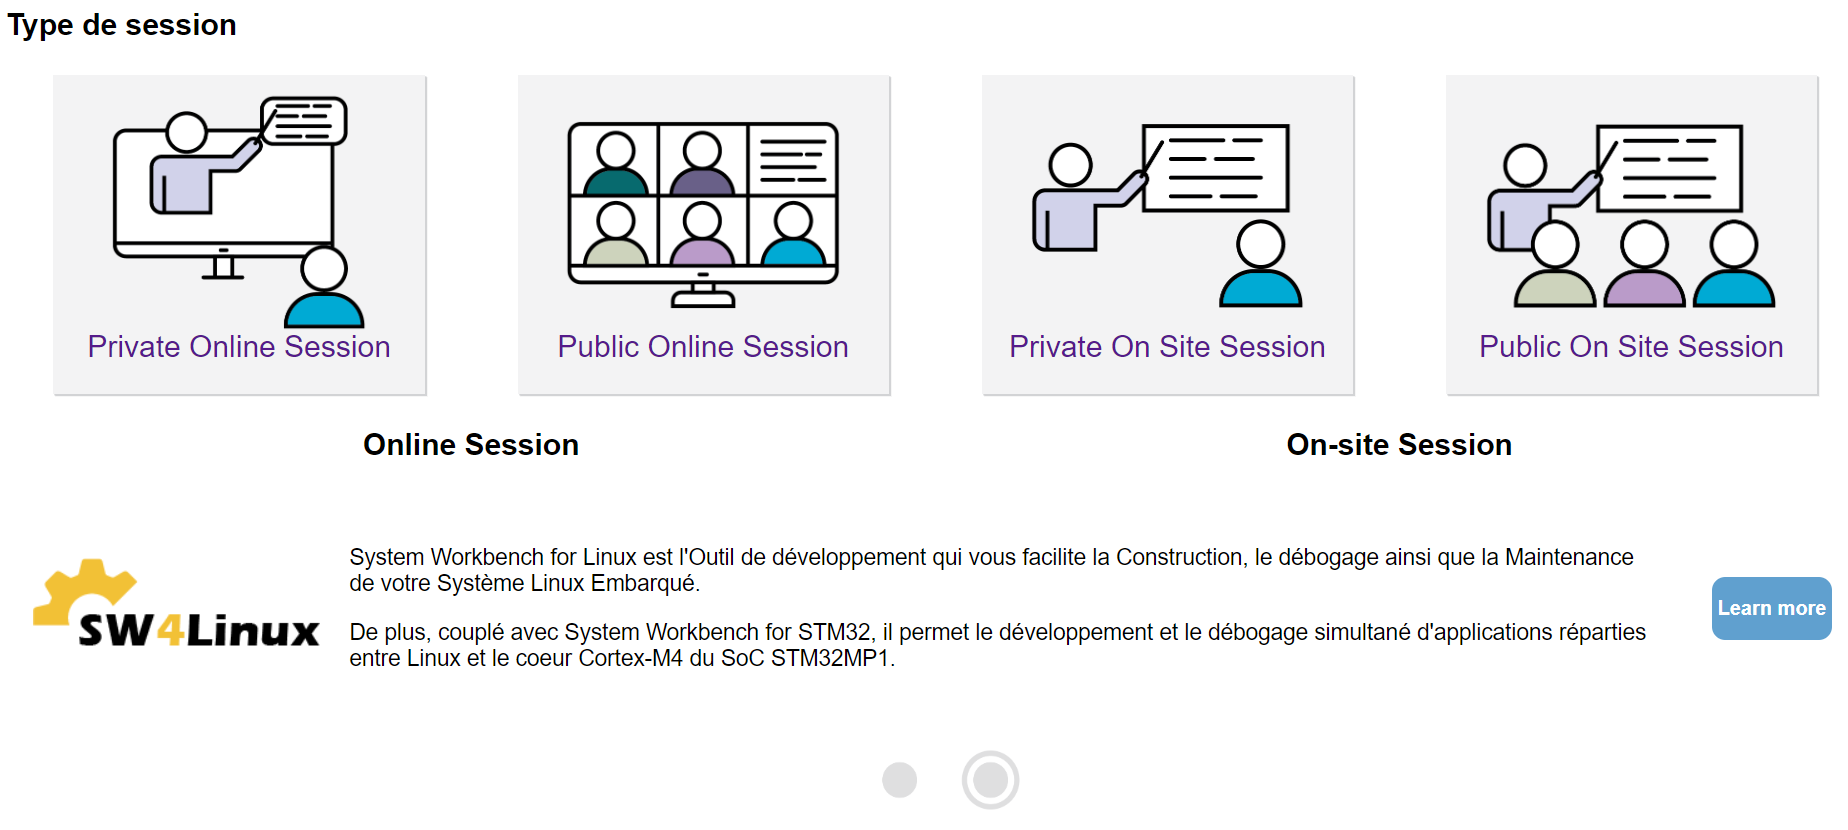
\includegraphics[width=\textwidth]{training 2.png}
    \caption{Website Mock-up - Training Page (2)}
    \label{training 2}
\end{figure}

\begin{figure}[h]
    \centering
    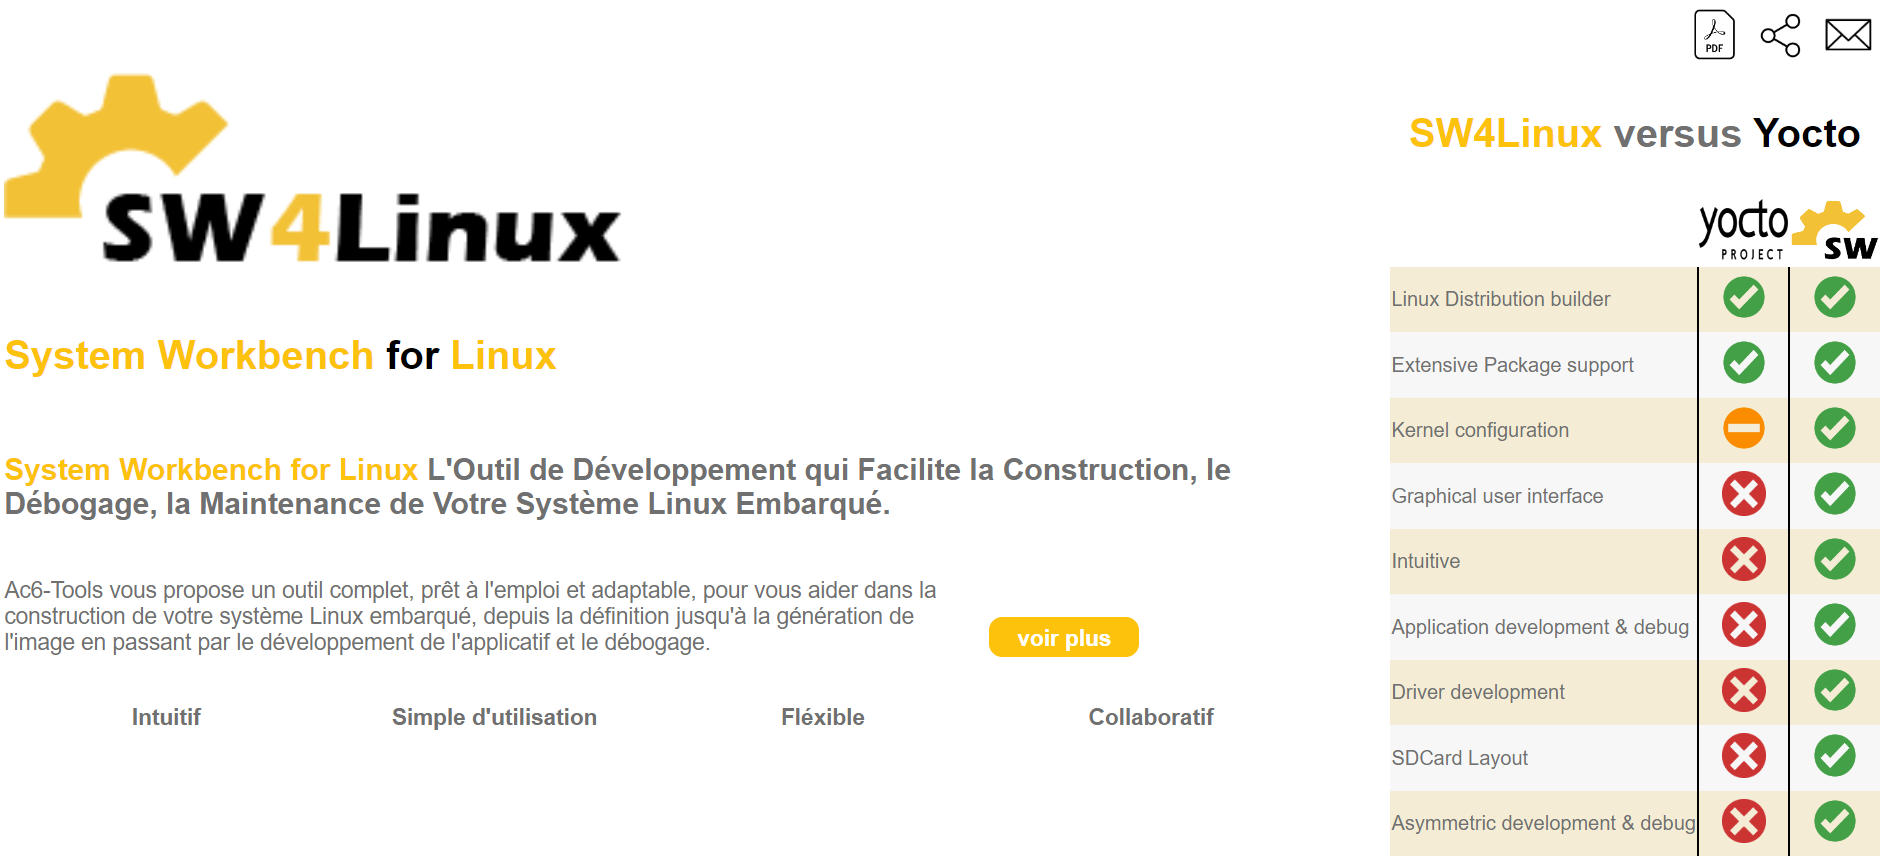
\includegraphics[width=\textwidth]{tools.png}
    \caption{Website Mock-up - System Workbench for Linux}
    \label{tools}
\end{figure}

\end{document}
